\chapter{Представление знаний с помощью графов знаний} \label{ch1}

% не рекомендуется использовать отдельную section <<введение>> после лета 2020 года
%\section{Введение. Сложносоставное название первого параграфа первой главы для~демонстрации переноса слов в содержании} \label{ch1:intro}


\section{Представление знаний}

Человеку свойственно понимать, рассуждать и интерпретировать знания. Знания, которые накапливаются со временем, позволяют людям выполнять
задачи. Аналогичная концепция уже очень давно является целью компьютерных наук и искусственного интеллекта, а способ обработки таких знаний
машинами заключается в представлении знаний. Представление знаний направлено на то, чтобы добавить следствие или рассуждения, лежащие в
основе рассматриваемого объекта. Этим объектом может быть конкретная деятельность, медицинский диагноз и т.д. Важно отметить, что
представление знаний - это не просто хранение данных в базе данных, но и способность учиться и совершенствовать эти знания, подобно тому, как
ведет себя человек. В своей работе "What is a Knowledge Representation?" Дэвис, Шроуб и Шоловиц выводят идею о том, что знания для субъекта
представлены самим субъектом и предполагаемыми отношениями, которые он имеет с другими субъектами, фактами, обстоятельствами и так далее.

Существует три основных способа представления знаний: логическое, семантическое и фреймовое. Семантические сети являются альтернативой
логическому представлению, в том смысле, что они представляют знания в виде графических сетей. Графическая сеть состоит из узлов,
представляющих объекты, и дуг, описывающих отношения между этими объектами. Пример на рис.1.1 визуализирует семантические сети.

\begin{figure}[ht!]
    \center
    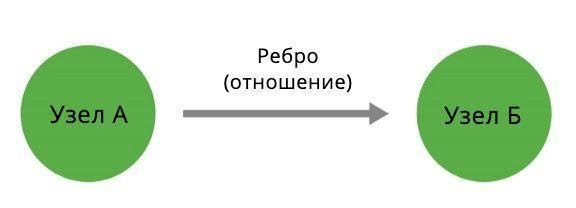
\includegraphics[scale=0.8]{my_folder/myimg//1}
    \caption{Пример семантической сети}
\end{figure}


\section{Графовое представление знаний}

Семантические сети были разработаны как техника представления знаний, чтобы проиллюстрировать, как концепции связаны друг с другом.
Семантические сети берут верх над логическими представлениями, потому что они более естественны и интуитивны, и обладают большей когнитивной
адекватностью по сравнению со своим логическим аналогом. Графы знаний — это форма семантических сетей, обычно ограниченная определенным
доменом, и управляемая как граф. Элринджер и Вёсс определяют графы знаний как знания, организованные таким образом, что машина может легко
понять и извлечь из них информацию, относящуюся к конкретной области, а также учиться на основе поглощенной информации, поэтому она лучше
справляется со связью вещей по мере поступления большего объема информации.

В отличие от обычной базы данных, которая наполняется и, в конечном счете, остается в состоянии покоя, граф знаний должен перепрофилироваться
и давать новые знания и умозаключения. Поскольку информация представлена в графовом виде, онтологии легко "расширяться и пересматриваться
по мере поступления новых данных". Онтология формально описывает типы, свойства и взаимосвязи между сущностями. Это набор аксиом (можно
считать принципами), определяющих знания в определенной области. Таким образом граф знаний является динамическим в том смысле, что сам граф
понимает, что связывает сущности, устраняя необходимость программировать каждый новый фрагмент информации вручную.


\section{Основные функции графа знаний}

Графы знаний могут иметь множество различных форм и могут быть представлены во многих вариациях, однако на рисунке 1.2 приведен общий
архитектурный обзор того, как работает граф знаний на основе обработки естественного языка.

\begin{figure}[ht!]
    \center
    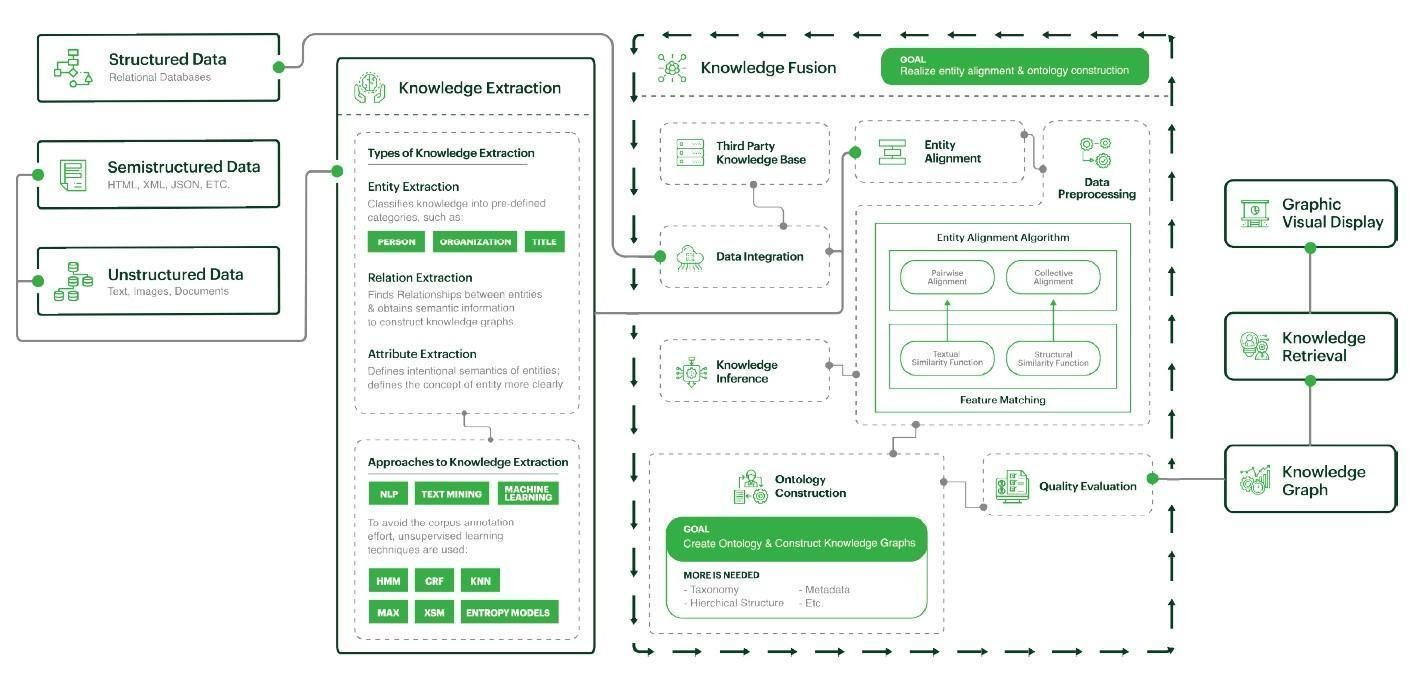
\includegraphics [scale=0.32] {my_folder/myimg//2}
    \caption{Архитектурный обзор того, как работает граф знаний на основе обработки естественного языка}
\end{figure}

\subsection{Источники данных}

Для построения графа знаний можно использовать различные источники данных, в том числе структурированные данные в виде реляционных баз
данных; полуструктурированные данные в виде HTML, JSON, XML и так далее, а также неструктурированные данные, такие как свободный текст,
изображения и документы. Во многих графах знаний используются данные из Википедии, а в специфических областях, таких как фильмы,
используются базы знаний, такие как IMDB.

\subsection{Извлечение данных}

После приема данных начинается процесс извлечения знаний. В ходе этого процесса из вводимых полуструктурированных и неструктурированных
данных извлекается информация, которая включает в себя сущности, связи и атрибуты. Это достигается с помощью методов обработки естественного
языка, извлечения текста и машинного обучения (как под наблюдением, так и без наблюдения).

Основная идея извлечения сущностей (иначе известного как распознавание сущностей) проста: учитывая некоторый текст, можно ли определить,
какие слова идентифицируют сущности определенных категорий? В общем, сущность может представлять человека, объект, место или вещь. Сущности
могут относиться к различным классам, которые также могут иметь подклассы. Например, классом сущности может быть "человек". Классы сущностей
"футболист", "танцор", "актер" могут относиться к классу сущностей "человек", так как все они являются разновидностью человека. Предложение
"Владимир Путин — один из президентов России" указывает на то, что сущность Владимир Путин относится к классу сущностей "президенты России".

После того, как все сущности извлечены, собирается информация об этих сущностях и их атрибутах. Сюда могут входить свойства сущностей, а
также отношения между ними. Например, сущность "человек" может быть связана с "местом рождения", "полом" и так далее. Иногда атрибут сущности
может описывать отношения между двумя сущностями или классами сущностей. Например, сущность "гольф" может быть ассоциирована с атрибутом
сущности "является подклассом" с классом сущности "спорт". Обычно, но не всегда, атрибут сущности является глаголом рассматриваемого предложения.

\subsection{Объединение знаний}

Идея слияния знаний состоит в том, чтобы объединить все базы знаний, поступающие из различных источников, чтобы получить всеобъемлющее
представление. Ее конкретные цели заключаются в реализации слияния сущностей и онтологического конструирования. Совмещение объектов (или
согласование объектов) должно быть связано с определением того, относятся ли "различные объекты к одним и тем же объектам в реальном мире".
Стандартизация данных является важным этапом в процессе согласования структур, поскольку она позволяет получить общее представление о данных.
Любое несоответствие данных разрешается на этом этапе. Граф знаний Linkedin является хорошим примером важности предварительной обработки и
стандартизации данных. Поскольку их сущности являются органическими сущностями, генерируемыми пользователями, многие из них включают
"недействительные или неполные атрибуты, бессмысленные имена или устаревшее содержимое". Может быть предпринято множество шагов, включая
создание кандидатов на сущности, разделение сущностей на кластеры на основе контекстов, в которых сущности появляются, удаление дублирующих
сущностей с помощью таких методов, как word2vec, и использование моделей машинного перевода для приведения всех сущностей к одному и тому же языку.

После того, как все данные интегрированы и согласованы, выполняется объединение записей, относящихся к одной и той же сущности, по парам и
группам. Сравнение парного сходства выполняется с использованием различных функций сходства текста, таких как косинусное сходство, а также
может интегрировать такие методы глубокого изучения, как word2vec, встраивание seq2seq и так далее. Групповое сопоставление осуществляется
с помощью функций структурного сходства, таких как распознавание образов и так далее. Вся эта работа приводит к созданию онтологии, которая
дополняется добавлением таксономии, иерархических структур, метаданных и так далее. для повышения качества графа знаний. Для обеспечения
общего качества графа знаний созданную онтологию сравнивают с отраслевыми схемами, такими как schema.org, и если она не соответствует
требованиям, то происходит итерация и усовершенствование процесса. Важно подчеркнуть важность итеративного характера этапа слияния знаний,
так как именно на этом этапе происходит основная часть моделирования.

\subsection{Хранение, извлечение и визуальное представление знаний}

После создания граф знаний может храниться в реляционной базе данных, базе данных NoSQL или графовой базе данных. Информация о всех данных
представлена в RDF (Resource Description Framework) формате, который основывается на триплетах. RDF триплет состоит из субъекта, предиката и
объекта, но в то же время к любому триплету может быть добавлена ещё одна ссылка для хранения метаданных.

В случае использования реляционной или NoSQL базы необходимы промежуточные шаги для трансформации данных в RDF граф, в то время как
использование графовой базы данных позволяет осуществлять взаимодействие с данными без дополнительной обработки. Для получения данных из RDF
графа чаще всего используется SPARQL — традиционный язык запросов для получения крупномасштабных графов знаний.

Визуализация большого количества графов знаний осуществляется через браузерные приложения, и остается одной из наиболее исследуемых тем в этой области.


\section{Использование графа знаний}

Рассмотрим основные направления использования графов знаний.

\subsection{Доступ к данным по API}

Прямой доступ к графу знаний с помощью простого поиска и запросов облегчает разработку приложений, в которых необходимо использовать данные
из нескольких источников. Наличие единого представления о структуре данных предприятия позволяет быстро разрабатывать новые приложения.
Одним из лучших способов достижения этой цели является разработка "ориентированного на данные API", в котором вызывающая сторона указывает
данные, которые ей нужны, вместо того чтобы разрабатывать API для конкретных случаев использования.

Чаще всего в качестве API для графов знаний используется GraphQL. GraphQL — это ориентированный на данные API, в котором модель графовой
информации может быть сглажена в JSON по запросу, так что не графовые приложения могут запрашивать графовые данные привычным и удобным способом.

В зависимости от случаев использования может также потребоваться создание API для специфических случаев использования. Чаще всего это касается
получения данных для аналитики и машинного обучения.

\subsection{Потоковые данные}

Используя системы потоковой обработки данных наподобие Apache Kafka Streams, можно устранить узкие места на этапах обработки входных данных
и поддержания графа в актуальном состоянии в режиме реального времени.

\subsection{Аналитика}

Учитывая, что граф знаний представляет собой полностью связное представление данных о предприятии, он, таким образом, является полномасштабным
источником данных для системы BI/MI (Business Intelligence / Management Information). Работа по сбору и связыванию данных абстрагируется на
графе, а архитектура BI/MI может быть упрощена для потребления информации из графа. Таким образом, граф знаний играет центральную роль в
создании отчетов, выполнении аналитических запросов и предоставлении визуализаций. Он также может быть источником информации для современных
поисковых решений на основе AI, которые используют тысячи параметров одновременно, чтобы показать "горячие точки" и отклонения, которые имеют значение.

\subsection{Машинное обучение}

Большая часть задач по сбору, связыванию и очистке данных выполняется самим графом, что позволяет упростить работу специалистов по работе с
данными. Также граф знаний может использоваться для обновления моделей и тренировочных наборов данных для машинного обучения. Если учесть,
что ключевой целью машинного обучения в бизнесе является прогнозирование, то граф знаний, который охватывает все бизнес-подразделения, является
ключевым источником входных данных для построения моделей.

Одной из общих задач машинного обучения, применяемой к графам является классификация узлов — обучение модели для определения того, к какому
классу принадлежит узел. Модели классификации узлов используются для предсказания несуществующего свойства узла на основе других свойств
узла. Несуществующее свойство узла представляет собой класс и называется целевым свойством. Указанные свойства узла используются в качестве
входных параметров. Модель классификации узлов не опирается на информацию о взаимосвязях, однако алгоритм встраивания узлов может встраивать
соседи узлов в качестве свойства, для передачи этой информации в модель Модели обучаются по частям входного графа и оцениваются по
определенным метрикам. Разделение графа на обучающий и тестовый графы выполняется внутренним алгоритмом, а тестовый граф используется для
оценки производительности модели.

Другой задачей машинного обучения, применяемой к графам является прогнозирование связей — построение модели для предсказания отсутствующих
связей в наборе данных или связей, которые, вероятно, будут формироваться в будущем. Обычно работа с прогнозированием связи подразделяется
на следующие этапы:

\begin{itemize}
    \item создание графов для обучения и тестирования;
    \item обучение и оценивание кандидатов-моделей;
    \item применение модели для прогнозирования.
\end{itemize}

Еще одной задачей машинного обучения, применяемой к графам является поиск сообществ. При исследовании сложных сетей считается, что сеть имеет
структуру сообщества, если узлы сети можно легко сгруппировать в наборы узлов таким образом, чтобы каждый набор узлов был плотно связан
внутренне. В конкретном случае поиска не пересекающихся сообществ это означает, что сеть естественным образом разделяется на группы узлов с
плотными внутренними связями и более узкие связи между группами. Но накладывающиеся друг на друга сообщества также допустимы. Более общее
определение основано на принципе, что пары узлов с большей вероятностью будут связаны, если они оба являются членами одного и того же
сообщества (сообществ), и с меньшей вероятностью будут связаны, если они не разделяют сообщества.

Поиск сообществ в произвольной сети может оказаться сложной вычислительной задачей. Количество сообществ, если таковые имеются, внутри сети,
как правило, неизвестно, и сообщества часто имеют неравные размеры и/или плотность. Однако, несмотря на эти трудности, было разработано и
использовано несколько методов поиска сообществ с разной степенью успеха:

\begin{itemize}
    \item метод наименьших разрезов;
    \item иерархическая кластеризация;
    \item алгоритм Гирван — Ньюмена;
    \item максимизация модульности;
    \item статический вывод.
\end{itemize}


\section{Выводы}

Графы знаний являются мощным инструментом, позволяющим полностью использовать графовую природу данных в самых различных направлениях —
начиная от мониторинга взаимодействия сотрудников внутри небольшого предприятия, заканчивая улучшением результатов поиска крупнейшей
поисковой системы Google.

На данный момент не существует единственного верного подхода для реализации графов знаний. Большинство различий заключается в выборе базы
данных, в которой будет осуществляться хранение графовых данных. Так, для работы таких основных функций как: получение данных из внешних
источников, извлечение и объединение данных - критическую роль играет поддержка хранения графовых структур на стороне базы данных и
возможности встроенного языка запросов. А для таких направлений использования графа знаний как: доступ к данным по API и подготовка данных
для аналитики и машинного обучения - критическую роль играет скорость сбора графовых данных на стороне базы и ориентированность встроенного
языка на выполнение запросов разной степени сложности. Именно поэтому перед построением графа знаний необходимо произвести исследования
различных типов баз данных по следующим направлениям:

\begin{itemize}
    \item исследование способов хранения графовых данных — в рамках которого будет определено насколько база данных ориентирована на хранение графовых данных, какие дополнительные действия необходимо произвести в случае отсутствия поддержки по умолчанию и какой размер памяти будет занимать загруженный граф;
    \item исследование функциональности и производительности языка запросов при вставке данных — в рамках которого будет определено насколько язык запросов ориентирован на вставку одиночных и множественных данных, а также время необходимое на совершение данных операций;
    \item исследование функциональности и производительности языка запросов при извлечении данных — в рамках которого будет определено насколько язык запросов ориентирован на извлечение данных по атрибутам и на основе графовых алгоритмов, а также время необходимое на совершение данных операций.
\end{itemize}


%\subsection{Название первого подпараграфа первого параграфа первой главы для~демонстрации переноса слов в содержании} % ~ нужен, чтобы избавиться от висячего предлога (союза) в конце строки
%
%Содержание первого подпараграфа первого параграфа первой главы.
%
%
%
%Одиночные формулы оформляют в окружении \texttt{equation}, например, как указано в следующей одиночной нумерованной формуле:
%%
%%
%\begin{equation}% лучше не оставлять пропущенную строку (\par) перед окружениями для избежания лишних отсупов в pdf
%\label{eq:Pi-ch1} % eq - equations, далее название, ch поставлено для избежания дублирования
%\pi \approx 3,141.
%\end{equation}
%%
%%
%\begin{figure}[ht!]
%	\center
%	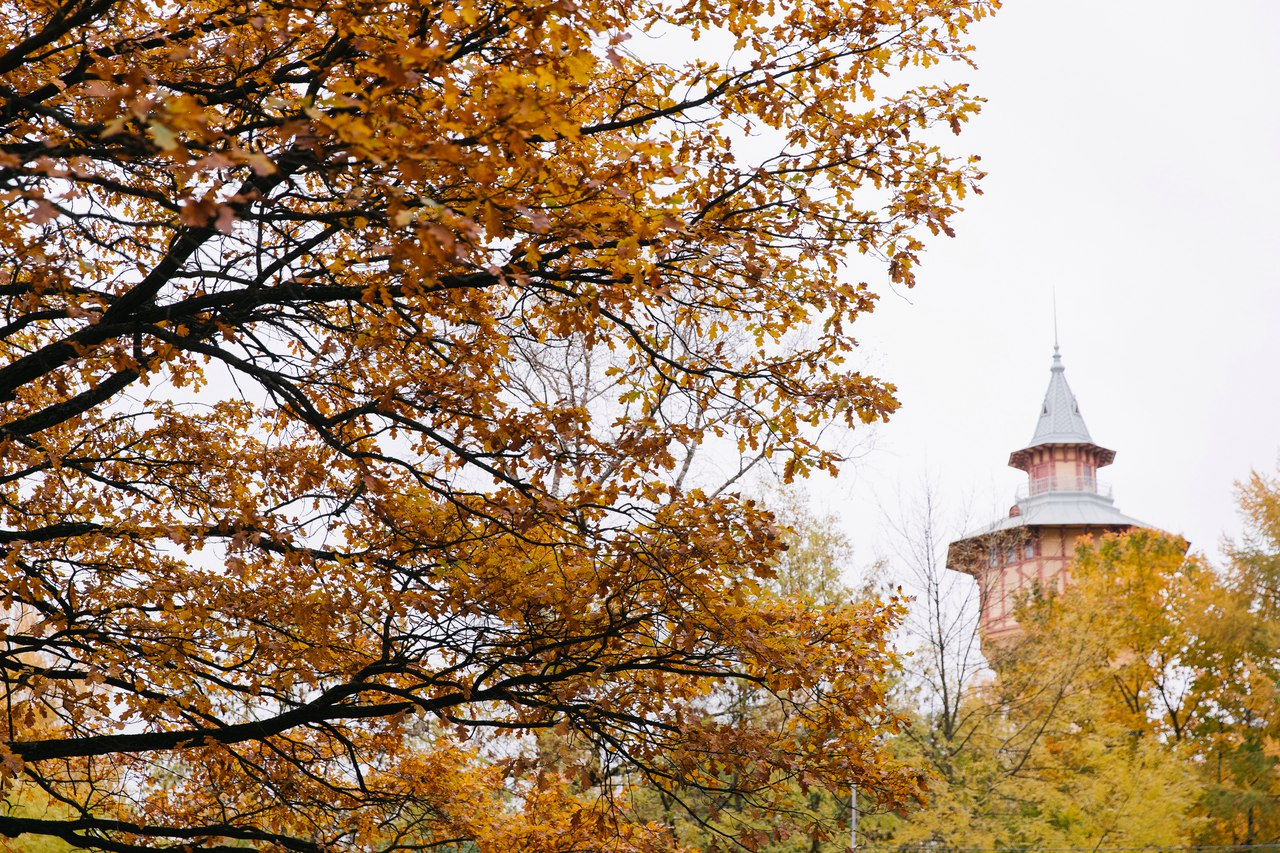
\includegraphics [scale=0.27] {my_folder/images//spbpu_hydrotower}
%	\caption{Вид на гидробашню СПбПУ \cite{spbpu-gallery}}
%	\label{fig:spbpu_hydrotower}
%\end{figure}
%%
%%
%%\begin{table} [htbp]% Пример оформления таблицы
%%	\centering\small
%%	\caption{Представление данных для сквозного примера по ВКР \cite{Peskov2004}}%
%%	\label{tab:ToyCompare}
%%		\begin{tabular}{|l|l|l|l|l|l|}
%%			\hline
%%			$G$&$m_1$&$m_2$&$m_3$&$m_4$&$K$\\
%%			\hline
%%			$g_1$&0&1&1&0&1\\ \hline
%%			$g_2$&1&2&0&1&1\\ \hline
%%			$g_3$&0&1&0&1&1\\ \hline
%%			$g_4$&1&2&1&0&2\\ \hline
%%			$g_5$&1&1&0&1&2\\ \hline
%%			$g_6$&1&1&1&2&2\\ \hline
%%		\end{tabular}
%%	\normalsize% возвращаем шрифт к нормальному
%%\end{table}
%
%
%% \firef{} от figure reference
%% \taref{} от table reference
%% \eqref{} от equation reference
%
%На \firef{fig:spbpu_hydrotower} изображена гидробашня СПбПУ, а в \taref{tab:ToyCompare} приведены данные, на примере которых коротко и наглядно будет изложена суть ВКР.
%
%
%\section{Название параграфа} \label{ch1:sec2}
%
%
%
%Формулы могут быть размещены в несколько строк. Чтобы выставить номер формулы напротив средней строки, используйте окружение \verb|multlined| из пакета \verb|mathtools| следующим образом \cite{Ganter1999}:
%%
%\begin{equation}
%\label{eq:fConcept-order-ch1}
%\begin{multlined}
%(A_1,B_1)\leq (A_2,B_2)\; \Leftrightarrow \\  \Leftrightarrow\; A_1\subseteq A_2\; \Leftrightarrow \\ \Leftrightarrow\; B_2\subseteq B_1.
%\end{multlined}
%\end{equation}
%
%
%Используя команду \verb|\labelcref| из пакета \verb|cleveref|, допустимо следующим образом оформлять ссылку на несколько формул:
%(\labelcref{eq:Pi-ch1,eq:fConcept-order-ch1}).
%%
%%
%На \firef{fig:spbpu_whitehall-three-photos} приведены три картинки под~общим номером и~названием, но с раздельной нумерацией подрисунков посредством пакета \verb|subcaption|.
%
\begin{figure}[!htbp]
	\adjustbox{minipage=1.3em,valign=t}{\subcaption{}\label{fig:spbpu_whitehall-a}}%
	\begin{subfigure}[t]{\dimexpr.3\linewidth-1.3em\relax}
		\centering
		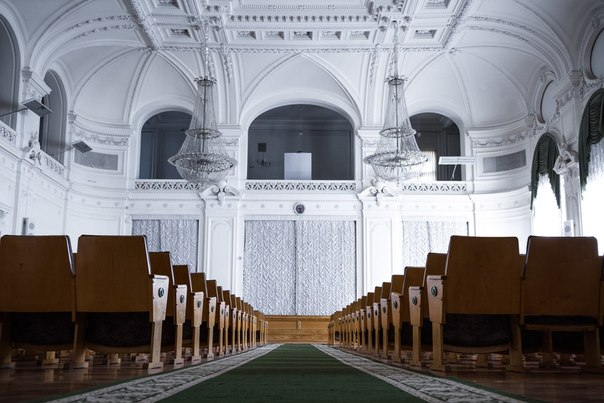
\includegraphics[width=.95\linewidth,valign=t]{my_folder/images//spbpu_whitehall}
	\end{subfigure}
	\hfill %выровнять
	\adjustbox{minipage=1.3em,valign=t}{\subcaption{}\label{fig:spbpu_whitehall-b}}%
	\begin{subfigure}[t]{\dimexpr.3\linewidth-1.3em\relax}
		\centering
		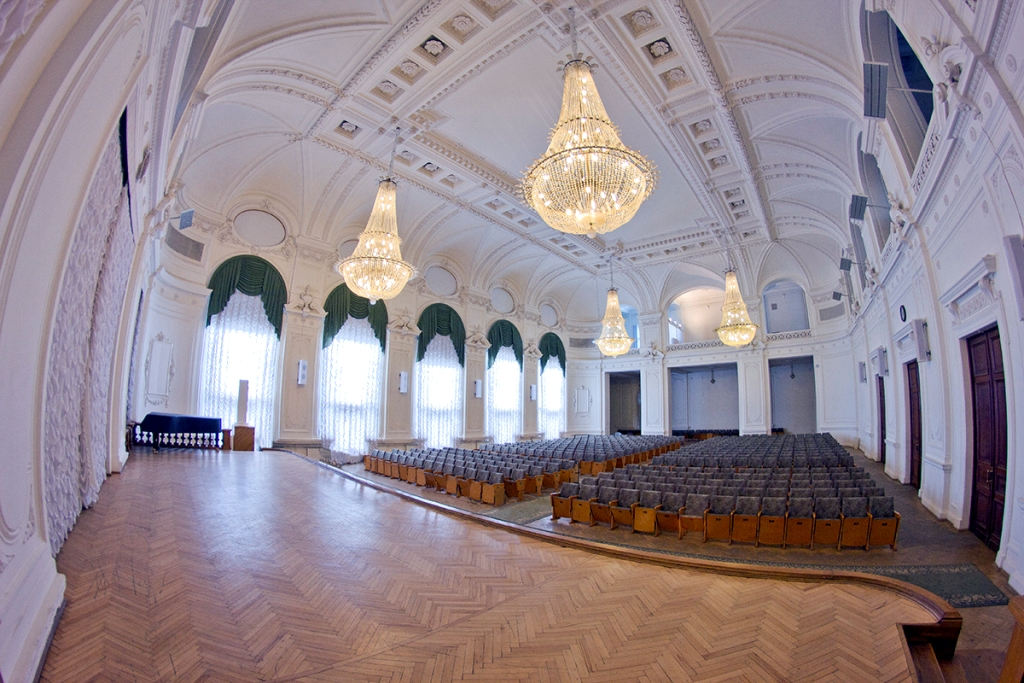
\includegraphics[width=.95\linewidth,valign=t]{my_folder/images//spbpu_whitehall_ligh}
	\end{subfigure}
	\hfill %выровнять
		\adjustbox{minipage=1.3em,valign=t}{\subcaption{}\label{fig:spbpu_whitehall-c}}%
	\begin{subfigure}[t]{\dimexpr.3\linewidth-1.3em\relax}
		\centering
		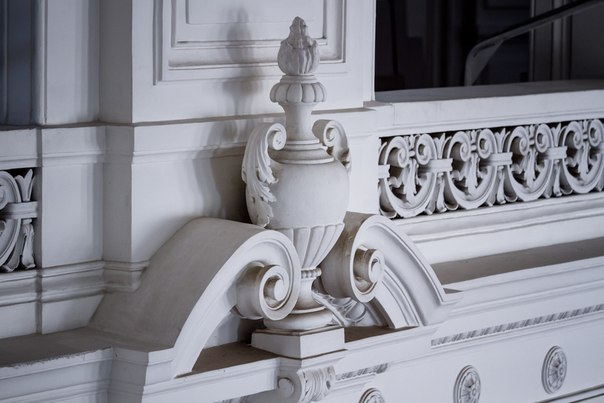
\includegraphics[width=.95\linewidth,valign=t]{my_folder/images//spbpu_whitehall_sculpture}
	\end{subfigure}%
\captionsetup{justification=centering} %центрировать
	\caption{Фотографии Белого зала СПбПУ \cite{spbpu-gallery}, в том числе: {\itshape a} --- со стороны зрителей; {\itshape b} --- со стороны сцены; {\itshape c} --- барельеф}\label{fig:spbpu_whitehall-three-photos}  
\end{figure}

Далее можно ссылаться на три отдельных рисунка: \firef{fig:spbpu_whitehall-a}, \firef{fig:spbpu_whitehall-b} и \firef{fig:spbpu_whitehall-c}. % пример подключения 3х иллюстрации в одном рисунке
%
%Пример ссылок \cite{Article,Book,Booklet,Conference,Inbook,Incollection,Manual,Mastersthesis,Misc,Phdthesis,Proceedings,Techreport,Unpublished,badiou:briefings}, а также ссылок с указанием страниц, на котором отображены номера страниц  \cite[с.~96]{Naidenova2017} или в виде мультицитаты на несколько источников \cites[с.~96]{Naidenova2017}[с.~46]{Ganter1999}. Часть библиографических записей носит иллюстративный характер и не имеет отношения к реальной литературе.
%
%
%
%%\FloatBarrier % заставить рисунки и другие подвижные (float) элементы остановиться
%
%\section{Выводы} \label{ch1:conclusion}
%
%Текст выводов по главе \thechapter.
%
%Кроме названия параграфа <<выводы>> можно использовать (единообразно по всем главам) следующие подходы к именованию последних разделов с результатами по главам:
%\begin{itemize}
%	\item <<выводы по главе N>>, где N --- номер соответствующей главы;
%	\item <<резюме>>;
%	\item <<резюме по главе N>>, где N --- номер соответствующей главы.
%\end{itemize}
%
%Параграф с изложением выводов по главе \textit{является обязательным}.

%% Вспомогательные команды - Additional commands
%
%\newpage % принудительное начало с новой страницы, использовать только в конце раздела
%\clearpage % осуществляется пакетом <<placeins>> в пределах секций
%\newpage\leavevmode\thispagestyle{empty}\newpage % 100 % начало новой страницы